\section{Absorption on phonons and acoustic modes}\label{sec:11.8}

A dark photon of mass \SI{36.35}{meV} that is absorbed in GaAs deposits its whole energy in one longitudinal optical phonon, and its momentum, $m_\phi v \approx \SI{46}{\micro eV}$, is a part in $10^{8}$ of the zone. Absorption samples the crystal at a single point, $\vect{q} = \vect{p}_\phi$ and $\omega = m_\phi$ (\cref{sec:8.2-absorption}), and below the electronic gap the only excitations at that point are the optical phonons at the zone center. For bosons of a neV or a \si{\micro eV} the picture changes again. Their de Broglie wavelength $2\pi/m_\phi v$, a kilometer at \SI{1}{\micro eV}, is larger than any detector, and the field is a classical wave that oscillates in phase over the whole body. What absorbs it is a normal mode of the body itself, at MHz in a millimeter crystal and at kHz in a ton-scale bar. A scalar coupled to electrons sees the electrons that a longitudinal phonon carries with each nucleus, and in GaAs, where the two sublattices carry nearly equal numbers per unit mass, its rate is a near-cancellation.

\subsection{Single-phonon absorption}\label{sec:11.8-single}

The absorption rate per quantum is the master formula \cref{eq:8.2-abs} at one point. Collect the couplings of the field into one row, $O_\phi = \sum_ag^\phi_aO_a(\vect{p}_\phi)$; then $\varGamma_{\mathrm{abs}} = S_{O_\phi O_\phi}(\vect{p}_\phi,\omega_\phi)/2\omega_\phi$, and in a cold insulator below the gap $S$ is the one-phonon structure factor. The kinematics leaves no choice of branch. An acoustic phonon of momentum $p_\phi$ has the energy $c_\nu p_\phi = c_\nu v\,m_\phi$, and absorbing the boson would need $c_\nu v = 1$, while sound speeds are $\sim 10^{-5}$ and $v \sim 10^{-3}$ in units of the speed of light. An optical phonon at $\vect{Q} = \vect{p}_\phi$ is the zone-center phonon to a part in $10^{15}$, since the dispersion starts at order $(p_\phi a)^2$. The momentum transfer is far below the \SI{0.05}{eV} at which the finite-$q$ structure of the longitudinal mode becomes visible (\cref{we:8-nucleon}), and the zone-center vertex is exact here. The finite-$q$ corrections of \cref{sec:11.2}, the piezoelectric charge of the acoustic branches and the dynamical quadrupoles, play no role.

For a row built from densities the one-phonon structure factor has the form of \cref{eq:11.1-S1} and \cref{eq:11.2-SZZ}: each sublattice contributes its displacement projected on $\vect{p}_\phi$, times a coupling per site. With $\omega_\phi \simeq m_\phi$ and $T = 0$,
\begin{equation}
  \varGamma_{\mathrm{abs}} = \frac{\pi}{2\Omega\,m_\phi}\sum_\nu\frac{\bigl|\sum_\kappa\vect{p}_\phi\cdot\mathcal{G}^\phi_\kappa\cdot\vect{e}_{\kappa\nu}(0)^*/\sqrt{M_\kappa}\bigr|^2}{\omega_\nu}\;\delta(m_\phi - \omega_\nu) ,
  \label{eq:11.8-Gamma}
\end{equation}
with $\omega_\nu$ and $\vect{e}_{\kappa\nu}(0)$ the zone-center phonons of the full dynamical matrix for the direction $\hat{\vect{p}}_\phi$, nonanalytic term included. The tensor $\mathcal{G}^\phi_\kappa$ is the coupling of the field to the motion of site $\kappa$, and finding it is the whole problem. The naive answer is the coefficient of each species times the number of particles that move with the nucleus. For the nucleons that number is fixed. For the electrons it is not, because how many electrons follow a nucleus depends on the macroscopic field that the motion itself creates.

The Born charge answers half of the question. By its definition in \cref{sec:5.5}, $Z^*_\kappa$ is the charge that moves with nucleus $\kappa$ at zero macroscopic field: the nuclear charge $Z_\kappa$ minus the electrons that follow. At zero field the electrons that follow thus number $Z_\kappa\mathbb{1} - Z^*_\kappa$, and this is the vertex of the electron density in the proper response. A longitudinal phonon, however, carries a macroscopic field, and the electrons respond to it as well. The screened response \cref{eq:8.4-rank1} adds that field, and \cref{we:8-nucleon} has done the algebra for a nucleon row. The electron row differs in one respect: it also correlates with the charge through the electrons alone, at fixed nuclei.

For any pair of rows, take frequencies near the optical phonons and neglect local fields. The screened response is then the rank-one form \cref{eq:8.4-rank1}, $R_{ab} = \tilde R_{ab} + v_{\mathrm{C}}\tilde R_{aZ}\tilde R_{Zb}/\varepsilon$ with $\varepsilon = 1 - v_{\mathrm{C}}\tilde R_{ZZ}$, built from the proper responses $\tilde R$. The proper response of rows $a$ and $b$ then has a phonon part and an electronic part,
\begin{equation*}
  \tilde R_{ab} = \frac{q^2}{\Omega}\,\vect{p}_a^{\mathrm{T}}\bigl(\omega^2 - D^{\mathrm{an}}\bigr)^{-1}\vect{p}_b + \chi_{ab} ,
\end{equation*}
with $\vect{p}_a$ the $3n$-vector of the proper site couplings of row $a$ divided by $\sqrt{M_\kappa}$ and projected on $\hat{\vect{q}}$, as in \cref{eq:11.2-eps}, and $\chi_{ab}$ the real response of the electrons at clamped nuclei. For the charge row, $\vect{p}_Z = \vect{p}$ is built from the Born charges and $v_{\mathrm{C}}\chi_{ZZ} = 1 - \varepsilon_\infty$. Write $x_a = (q^2/\Omega)\,\vect{p}_a^{\mathrm{T}}(\omega^2 - D^{\mathrm{an}})^{-1}\vect{p}$ and $x = x_Z$, so that $\varepsilon = \varepsilon_\infty - v_{\mathrm{C}}x$. The full phonon propagator $(\omega^2 - D^{\mathrm{an}} - \vect{b}\vect{b}^{\mathrm{T}})^{-1}$, with $\vect{b}\vect{b}^{\mathrm{T}}$ the nonanalytic term of \cref{eq:11.2-SM}, follows from the Sherman--Morrison identity, and between rows it gives $x_ax_b$-type terms:
\begin{equation*}
  \frac{q^2}{\Omega}\,\vect{p}_a^{\mathrm{T}}\bigl(\omega^2 - D^{\mathrm{an}} - \vect{b}\vect{b}^{\mathrm{T}}\bigr)^{-1}\vect{p}_b = \frac{q^2}{\Omega}\,\vect{p}_a^{\mathrm{T}}\bigl(\omega^2 - D^{\mathrm{an}}\bigr)^{-1}\vect{p}_b + \frac{v_{\mathrm{C}}\,x_ax_b}{\varepsilon_\infty - v_{\mathrm{C}}x} .
\end{equation*}
Insert $\tilde R_{aZ} = x_a + \chi_{aZ}$ into \cref{eq:8.4-rank1} and expand the product $(x_a + \chi_{aZ})(x_b + \chi_{bZ})$. The $x_ax_b$ term is the one just written. The terms linear in $\chi$ and the $\chi\chi$ term are reproduced by shifting each vertex by $\lambda_a\vect{p}$ with $\lambda_a = v_{\mathrm{C}}\chi_{aZ}/\varepsilon_\infty$, since $(q^2/\Omega)\vect{p}_a^{\mathrm{T}}(\omega^2 - D^{\mathrm{an}} - \vect{b}\vect{b}^{\mathrm{T}})^{-1}\vect{p} = \varepsilon_\infty x_a/\varepsilon$ by the same identity; what remains of the $\chi\chi$ term is a real constant. The result is exact within the rank-one form:
\begin{equation}
  R_{ab} = \frac{q^2}{\Omega}\,\vect{p}'^{\mathrm{T}}_a\bigl(\omega^2 - D^{\mathrm{an}} - \vect{b}\vect{b}^{\mathrm{T}}\bigr)^{-1}\vect{p}'_b + \chi_{ab} + \frac{v_{\mathrm{C}}\chi_{aZ}\chi_{Zb}}{\varepsilon_\infty} ,
  \qquad \vect{p}'_a = \vect{p}_a + \frac{v_{\mathrm{C}}\chi_{aZ}}{\varepsilon_\infty}\,\vect{p} .
  \label{eq:11.8-shift}
\end{equation}
The transverse poles are gone, the phonons are those of the full dynamical matrix, and each row keeps its own vertex, shifted along the Born-charge vector by its electronic correlation with the charge. The constant is real and does not absorb. For the electron density, $n_Z = -n_e + \sum_\kappa Z_\kappa n_\kappa$ gives $\chi_{eZ} = -\chi_{ee} = -\chi_{ZZ}$, so that $v_{\mathrm{C}}\chi_{eZ} = \varepsilon_\infty - 1$, and the shift adds $(1 - 1/\varepsilon_\infty)Z^*_\kappa$ to the proper vertex $Z_\kappa\mathbb{1} - Z^*_\kappa$.
\begin{keyresult}[Site coupling of a density row at the longitudinal pole]
A field that couples to $\sum_\kappa g^\phi_{n_\kappa}n_\kappa + g^\phi_{n_e}n_e$ creates the zone-center phonons of \cref{eq:11.8-Gamma} with the site couplings
\begin{equation}
  \mathcal{G}^\phi_\kappa = g^\phi_{n_\kappa}\mathbb{1} + g^\phi_{n_e}\Bigl(Z_\kappa\mathbb{1} - \frac{Z^*_\kappa}{\varepsilon_\infty(\hat{\vect{p}}_\phi)}\Bigr) ,
  \label{eq:11.8-G}
\end{equation}
for $\omega$ far below the gap, without local fields, and in the harmonic lattice. A longitudinal phonon carries $Z_\kappa - Z^*_\kappa/\varepsilon_\infty$ electrons with nucleus $\kappa$.
\end{keyresult}
\noindent The total charge, the nucleon number and the electron density each test \cref{eq:11.8-G}. For the total charge, $g^\phi_{n_e} = -\lambda$ and $g^\phi_{n_\kappa} = \lambda Z_\kappa$, and the nuclear charge cancels to leave $\lambda Z^*_\kappa/\varepsilon_\infty$, the screened Born charge of \cref{eq:11.2-SZZ}. For the nucleons, $g^\phi_{n_e} = 0$ and the vertex is the bare coefficient, unscreened, as \cref{we:8-nucleon} found. For the electrons alone the vertex is new. In the longitudinal wave the macroscopic field is $-\vect{P}/\varepsilon_\infty$, the electrons polarize in it, and they move another $Z^*_\kappa(1 - 1/\varepsilon_\infty)$ along with the nucleus, in addition to the $Z_\kappa - Z^*_\kappa$ that follow at zero field.

Optical phonons do not move the center of mass, $\sum_\kappa\sqrt{M_\kappa}\,\vect{e}_{\kappa\nu}(0) = 0$, and by the coupling-to-mass cancellation of \cref{sec:11.6-random} the sum in \cref{eq:11.8-Gamma} is unchanged when $\mathcal{G}^\phi_\kappa \to \mathcal{G}^\phi_\kappa - \lambda M_\kappa\mathbb{1}$ for any $\lambda$: a coupling proportional to the mass excites no optical phonon at all~\cite[Eq.~(44)]{mitridate2024effective}. What \cref{eq:11.8-Gamma} measures is how far the site couplings deviate from proportionality to the masses. For two atoms in the cell, with the longitudinal eigenvector of \cref{sec:11.2}, $\vect{e}_1 = (M_2/M_{\mathrm{cell}})^{1/2}\hat{\vect{p}}_\phi$ and $\vect{e}_2 = -(M_1/M_{\mathrm{cell}})^{1/2}\hat{\vect{p}}_\phi$, the sum collapses to $p_\phi\,\mu_{\mathrm{red}}^{1/2}\,d$ with the mass-weighted difference
\begin{equation}
  d = \frac{\mathcal{G}^\phi_1}{M_1} - \frac{\mathcal{G}^\phi_2}{M_2} ,
  \label{eq:11.8-d}
\end{equation}
in a cubic crystal, where the tensors are scalars. Only the longitudinal mode couples, since $\vect{p}_\phi\cdot\vect{e}$ vanishes for the transverse ones.

The rate takes a compact form through the loss function. By \cref{eq:11.2-onebranch} the longitudinal line of $L$ has the weight $\pi e^2Z^{*2}/(2\Omega\mu_{\mathrm{red}}\varepsilon_\infty^2\omega_{\mathrm{L}})$. Dividing \cref{eq:11.8-Gamma} by it, averaging $p_\phi^2 = m_\phi^2v^2$ over the halo and multiplying by $\rho_\chi/m_\phi\rho_T$,
\begin{equation}
  \mathcal{R} = \frac{\rho_\chi}{\rho_T}\,\frac{\langle v^2\rangle}{e^2}\Bigl(\frac{\varepsilon_\infty\,\mu_{\mathrm{red}}\,d}{Z^*}\Bigr)^2L(m_\phi) .
  \label{eq:11.8-Rscalar}
\end{equation}
In the one-branch crystal, with the damping carried by the phonon propagator, \cref{eq:11.8-shift} makes the full response of any density row proportional to $L(\omega)$ at every frequency, not only at the pole. The line shape is that of the loss function, peaked at $\omega_{\mathrm{L}}$, with no feature at $\omega_{\mathrm{T}}$. For a coupling proportional to the charge the bracket is one, and \cref{eq:11.8-Rscalar} is the photon-like rate of Mitridate and collaborators~\cite[Eq.~(42)]{mitridate2024effective}. Compared with the dark photon below, it carries $\langle v^2\rangle$, since a scalar couples to a density, whose matrix elements vanish as $p_\phi \to 0$. For the standard halo of \cref{sec:1.2}, $\langle v^2\rangle^{1/2} = \SI{379}{km/s}$. A photon-like scalar then reaches the dark-photon sensitivity at $g = \zeta e/\langle v^2\rangle^{1/2} = 240\,\zeta$.

For a scalar that couples to nucleon number the bracket is $\varepsilon_\infty\mu_{\mathrm{red}}d_N/Z^*$, with $d_N$ the difference of nucleon number per mass between the two species, $2.6\times10^{-5}$ per u in GaAs (\cref{we:8-nucleon}). The bracket is $4.8\times10^{-3}$, and the rate is $2\times10^{-5}$ of the photon-like one. Masses are nearly proportional to nucleon numbers, and the coupling-to-mass cancellation is nearly complete. In a crystal of mixed isotopes the cancellation fails site by site, the translation symmetry that selects the zone center is broken, and the absorption spreads over the whole phonon band (\cref{sec:11.6}).

A dark photon does not couple to a density. At rest it couples to the current, with any of three polarizations, and its rate per particle is $\varGamma_{\mathrm{net}} = \zeta^2m_\phi L(m_\phi)$ with the total dielectric function (\cref{sec:10.7-darkphoton}), the loss function again, now without the factor $v^2$. Why a transverse field excites the longitudinal phonon is the physics of the phonon polariton (\cref{sec:5.5}). The photon of the crystal and its transverse optical phonon mix into two branches near $Q \sim \varepsilon_0^{1/2}\omega_{\mathrm{T}}$, about \SI{0.12}{eV} in GaAs. The upper branch starts at $Q = 0$ at the zero of $\varepsilon$, which is $\omega_{\mathrm{L}}$; the lower one starts at zero frequency. The dark photon sits at $Q = p_\phi$, some 2600 times below the crossover, where the upper branch is flat at $\omega_{\mathrm{L}}$ and the distinction between transverse and longitudinal has disappeared: at $Q \to 0$ a cubic crystal has $\varepsilon^{\mathrm{T}} = \varepsilon$ (\cref{eq:4.4-ET}). With the line of \cref{eq:11.2-Ipol}, the rate integrated over the mass is
\begin{equation}
  \int\dd m_\phi\;\mathcal{R} = \frac{\rho_\chi}{\rho_T}\,\zeta^2\,\mathcal{I}_{\mathrm{pol}} ,
  \label{eq:11.8-Rint}
\end{equation}
the band integral of \cref{sec:11.2}, independent of the widths of the lines. Dark-photon absorption is single-phonon scattering through a dark photon, read at $q \to 0$.

\begin{limitbox}[Single-phonon absorption][lim:11.8a]
A boson absorbed on optical phonons has the rate $\varGamma_{\mathrm{abs}} = (\pi/2\Omega m_\phi)\sum_\nu|\sum_\kappa\vect{p}_\phi\cdot\mathcal{G}^\phi_\kappa\cdot\vect{e}^*_{\kappa\nu}(0)/\sqrt{M_\kappa}|^2\delta(m_\phi - \omega_\nu)/\omega_\nu$, \cref{eq:11.8-Gamma}~\cite[Eqs.~(2), (7), (14), (16)]{mitridate2024effective}. For a dark photon it is $\mathcal{R} = (\rho_\chi/\rho_T)\zeta^2\,\Imag[-1/\varepsilon(m_\phi)]$~\cite[Eqs.~(2), (3)]{knapen2018detection}, and for scalars \cref{eq:11.8-Rscalar} with the site couplings \cref{eq:11.8-G}.
\par\smallskip
{\centering
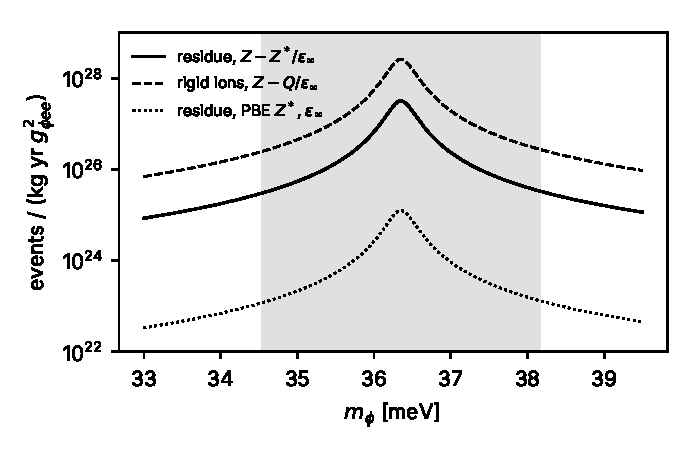
\includegraphics[width=0.8\linewidth]{figures/ch11/limit11_8a.pdf}
\captionof{figure}{Absorption of a scalar coupled to electrons in GaAs, events per kilogram-year and per $g_{\phi ee}^2$, against $m_\phi$, from \cref{eq:11.8-Rscalar}. Solid: site couplings $Z_\kappa - Z^*_\kappa/\varepsilon_\infty$ with $Z^* = 2.11$ and $\varepsilon_\infty = 10.88$ (\cref{we:5-lst}); a change of $Z^*/\varepsilon_\infty$ by $\pm\SI{1}{\percent}$ moves it by $\pm9\,\%$, less than the width of the line on this scale. Dotted: site couplings $Z_\kappa - Z^*_\kappa/\varepsilon_\infty$ with the PBE values $Z^* = 2.094$ and $\varepsilon_\infty = 13.70$ of \cref{sec:5.5}, 250 times lower. Loss function of one damped branch with $\omega_{\mathrm{T}} = 33.62$, $\omega_{\mathrm{L}} = \SI{36.35}{meV}$ and widths set to \SI{1}{\percent} of each frequency~\cite[Sect.~III\,A]{mitridate2024effective}; standard halo of \cref{sec:1.2}, $\langle v^2\rangle^{1/2} = \SI{379}{km/s}$, $\rho_T = \SI{5.361}{g.cm^{-3}}$. Gray: $|m_\phi - \omega_{\mathrm{L}}| < 5\gamma_{\mathrm{L}}$, where a line of constant width describes the phonon.}\label{fig:11-limit-8a}
\par}
\smallskip
Where the mass-weighted difference $d$ is small against each of its terms, the corrections that \cref{eq:11.8-G} drops are no longer small against the rate, and the formula fixes only its order of magnitude.
\end{limitbox}

\subsection{The near-cancellation in GaAs}\label{sec:11.8-gaas}

A scalar that couples to electrons through $g_{\phi ee}$ acts on the row $-g_{\phi ee}n_e$ (\cref{eq:8.1-scalar}), so that $g^\phi_{n_e} = -g_{\phi ee}$ and $g^\phi_{n_\kappa} = 0$, and by \cref{eq:11.8-G} each site contributes $Z_\kappa - Z^*_\kappa/\varepsilon_\infty$ electrons. GaAs is the obvious target, polar and well measured, and it turns out to be close to the worst case.

\begin{workedexample}{The electron-coupled scalar in GaAs}\label{we:11-gaas}
We take the inputs of \cref{sec:11.2}: $Z^* = 2.11$ from the splitting and the measured $\varepsilon_\infty = 10.88$, so that $Z^*/\varepsilon_\infty = 0.1939$, with $Z^*_{\mathrm{Ga}} = +Z^*$ and $Z^*_{\mathrm{As}} = -Z^*$; atomic numbers 31 and 33; mean atomic masses \SI{69.723}{u} and \SI{74.9216}{u}; $\mu_{\mathrm{red}} = \SI{36.11}{u}$.

\emph{Site couplings.} Gallium carries $31 - 0.1939 = 30.806$ electrons and arsenic $33 + 0.1939 = 33.194$, and each site couples with $-g_{\phi ee}$ times its count.

\emph{Mass-weighted difference.} Split \cref{eq:11.8-d} into its two parts. The nuclear charges per unit mass are $Z_{\mathrm{Ga}}/M_{\mathrm{Ga}} = 0.44462$ and $Z_{\mathrm{As}}/M_{\mathrm{As}} = 0.44046$ per u, and their difference is $+4.16\times10^{-3}$. The Born charges contribute $-(Z^*/\varepsilon_\infty)(1/M_{\mathrm{Ga}} + 1/M_{\mathrm{As}}) = -0.1939 \times 0.02769 = -5.37\times10^{-3}$. The sum is $d = -1.21\times10^{-3}$ per u, times $-g_{\phi ee}$. The two terms are 3.4 and 4.4 times larger than their sum.

\emph{Rate.} The bracket of \cref{eq:11.8-Rscalar} is $\varepsilon_\infty\mu_{\mathrm{red}}d/Z^* = 10.88 \times 36.11 \times 1.214\times10^{-3}/2.11 = 0.226$, and its square is $0.051$. An electron-coupled scalar is absorbed in GaAs at \SI{5}{\percent} of the rate of a photon-like scalar of the same coupling.

\emph{Sensitivity.} Since the Born-charge term is 4.4 times $|d|$, a fractional change of $Z^*/\varepsilon_\infty$ changes $d$ 4.4 times as much and the rate 8.8 times as much. The splitting route of \cref{sec:11.2-split} fixes $Z^*/\varepsilon_\infty$ to \SI{1.0}{\percent}, and these inputs limit the rate to \SI{9}{\percent}. Exact cancellation would need $Z^*/\varepsilon_\infty = 0.1501$. The values $Z^* = 2.16$ and $\varepsilon_\infty = 10.9$, also found in the literature, would give $d = -1.33\times10^{-3}$, a rate \SI{20}{\percent} higher.
\end{workedexample}

At the line center, with widths of \SI{1}{\percent}, three events in a kilogram-year need $g_{\phi ee} = 3.1\times10^{-14}$. III--V crystals, whose neighbors in the periodic table have nearly equal charge per mass, suppress the absorption of an electron-coupled scalar.

The kinetic energy of the core electrons, the isotopic masses and the frequency dependence of the electronic response are left out of \cref{eq:11.8-G}; each is small in absolute terms but not against $d$. The scalar density of an electron is its number density times $1 - v^2/2$ (\cref{eq:8.1-scalar}), and the core electrons that ride with a nucleus move fast. Their kinetic-energy row enters through the same factor $\ii\vect{p}_\phi\cdot\vect{u}_\kappa$ as their density, and it reduces the electrons each site carries by $\langle\mathcal{T}\rangle_\kappa/m_e$, the kinetic energy of those electrons over the electron mass. By the virial theorem this is the binding energy of the atom over $m_e$, tens of keV over \SI{511}{keV}, of order 0.1 for gallium and arsenic. As a parametric estimate, its mass-weighted difference between the two sites is $\Delta d \approx +1.2\times10^{-4}$ per u, a tenth of $d$ and of the opposite sign, so that it lowers $|d|$ by about \SI{10}{\percent} and the rate by about \SI{19}{\percent}. No calculation has included it yet, and \cref{sec:11.9} carries it as a nuisance. The masses enter at the same level: \SI{0.01}{u} on the mean mass of gallium moves $d$ by \SI{5}{\percent}, so an isotopically enriched crystal must use its own masses. The frequency dependence of the electronic response, of relative order $(\omega_{\mathrm{L}}/\Eg)^2 = 6\times10^{-4}$ (\cref{sec:11.2}), is amplified by 4.4 to \SI{0.3}{\percent} of $d$ and is negligible.

Density-functional perturbation theory delivers $Z^*$ robustly, to a percent, and $\varepsilon_\infty$ poorly. With the PBE values of \cref{sec:5.5}, $Z^* = 2.094$ and $\varepsilon_\infty = 13.70$, the ratio $Z^*/\varepsilon_\infty = 0.153$ lies within \SI{2}{\percent} of exact cancellation, $d = -7.6\times10^{-5}$ per u, and the rate falls by a factor of 250 (the dotted curve of \cref{lim:11.8a}). The test of the computed values against the measured splitting, \cref{eq:E.4-LOTO}, matters more here than any convergence parameter, and the measured splitting with \cref{eq:11.2-Zeps} is the safer input; the phonon widths come from three-phonon perturbation theory (\cref{sec:5.7}).

\subsection{Dark photons in GaAs and sapphire}\label{sec:11.8-dp}

For a dark photon the vertex is the screened Born charge, there is no cancellation, and the rate is the measured or computed loss function, $\mathcal{R} = (\rho_\chi/\rho_T)\zeta^2L(m_\phi)$ (\cref{eq:10.7-dp}). Two numbers characterize each line: its area, which is fixed by the band integral \cref{eq:11.8-Rint}, and its width, which is not. For GaAs, $\mathcal{I}_{\mathrm{pol}} = \SI{0.759}{meV}$ from the splitting (\cref{we:11-ipol}), and a Lorentzian of full width $\gamma_{\mathrm{L}}$ peaks at $L = 2\mathcal{I}_{\mathrm{pol}}/\pi\gamma_{\mathrm{L}}$. A width of \SI{1}{\percent} of the frequency leads to $L = 1.33$ at the center, ten times narrower gives 13.3, and the area stays at \SI{0.76}{meV}. The reach on the line center scales as $\gamma_{\mathrm{L}}^{1/2}$, while the reach averaged over a scan of masses depends only on the area.

\begin{figure}[tbp]
  \centering
  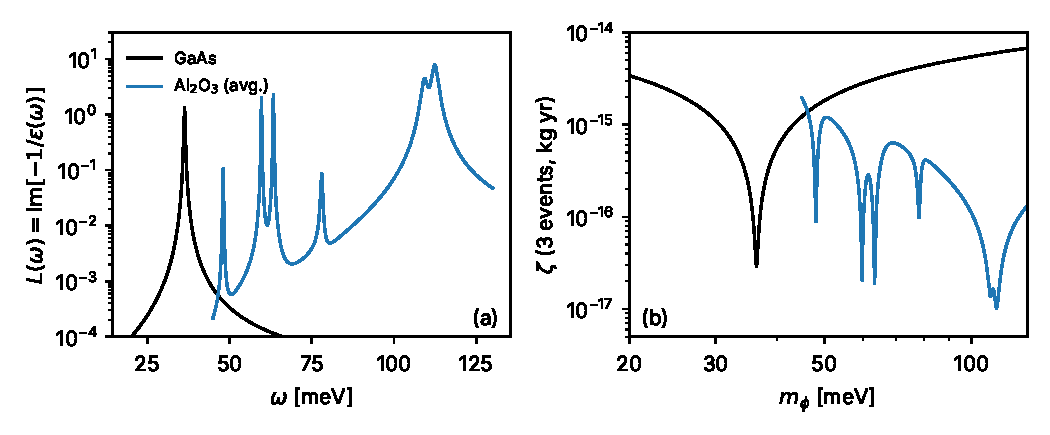
\includegraphics[width=\linewidth]{figures/ch11/fig11_8.pdf}
  \caption{Absorption of dark-photon dark matter on single optical phonons. (a) Loss function $L = \Imag[-1/\varepsilon(\omega)]$ at $q \to 0$ from the damped factorized dielectric function $\varepsilon_\infty\prod_\nu(\omega_{\mathrm{L}\nu}^2 - \omega^2 - \ii\omega\gamma_{\mathrm{L}\nu})/(\omega_{\mathrm{T}\nu}^2 - \omega^2 - \ii\omega\gamma_{\mathrm{T}\nu})$. GaAs (black): $\omega_{\mathrm{T}} = 33.62$, $\omega_{\mathrm{L}} = \SI{36.35}{meV}$, $\varepsilon_\infty = 10.88$, so that the line carries the splitting weight $(1 - \omega_{\mathrm{T}}^2/\omega_{\mathrm{L}}^2)/\varepsilon_\infty = 0.0133$ (\cref{sec:11.2}), with an assumed width of \SI{1}{\percent} of each frequency. Sapphire (blue): the frequencies and \SI{77}{K} widths of Ref.~\cite[Table~II]{griffin2018directional} for the ordinary and extraordinary rays, as listed in \cref{lim:10.7a}, and $\varepsilon_\infty = 3.2$; averaged over polarizations as $\frac23L_{\mathrm{o}} + \frac13L_{\mathrm{e}}$~\cite[Eq.~(40)]{griffin2018directional}; drawn above \SI{45}{meV}, since below the lowest transverse line the model gives $|L| < 10^{-4}$ of the wrong sign. (b) Kinetic mixing $\zeta$ for three events in one kilogram-year without background, $\mathcal{R} = (\rho_\chi/\rho_T)\zeta^2L(m_\phi)$, with $\rho_\chi = \SI{0.3}{GeV.cm^{-3}}$ and $\rho_T = 5.361$ and \SI{3.98}{g.cm^{-3}}. Single-phonon lines only: the multiphonon absorption between them and the electronic absorption above the gap are not included.}
  \label{fig:11-dpabs}
\end{figure}

\Cref{fig:11-dpabs} shows both crystals. GaAs has one line, and three events in a kilogram-year reach $\zeta = 2.9\times10^{-17}$ at its center. Sapphire has six polar branches between the two polarizations. The strongest is the collective top branch of the ordinary ray, at \SI{112.4}{meV}, which carries \SI{95}{\percent} of the ordinary weight (\cref{sec:11.2-band}). With its measured \SI{77}{K} width of \SI{2.0}{meV} it reaches $\zeta = 1.0\times10^{-17}$, and the lines at 59.7 and \SI{63.3}{meV} reach $2\times10^{-17}$. Per unit mass the band integral of sapphire is 64 times that of GaAs, $\SI{35.9}{meV}/\SI{3.98}{g.cm^{-3}}$ against $\SI{0.759}{meV}/\SI{5.361}{g.cm^{-3}}$; here \SI{35.9}{meV} is the polarization average $\frac23$ ordinary $+ \frac13$ extraordinary of the absorbed field, while the ordinary ray alone gives the \SI{36.3}{meV} of \cref{sec:11.2-band}. The widths are the weak input. Those of sapphire were measured at \SI{77}{K}, and at millikelvin temperatures the anharmonic part, the thermal part of \cref{eq:5.7-gamma}, shrinks while the spontaneous decay stays, so the lines should narrow by a factor of order one~\cite{griffin2018directional}. Between the lines the absorption is multiphonon, which the measured $\varepsilon$ contains and the factorized model does not, and it fills the gaps of \cref{fig:11-dpabs}b~\cite{knapen2018detection,griffin2018directional}.

\subsection{Acoustic modes of a finite body}\label{sec:11.8-bar}

The lowest thickness mode of a quartz plate \SI{1}{mm} thick rings at about \SI{3}{MHz}, an energy of \SI{12}{neV}. A dark photon of that mass has a de Broglie wavelength of order \SI{100}{km} and stays coherent for a fraction of a second, $t_{\mathrm{coh}} = 1/m_\phi v_0^2$, which is \SI{1.04}{ms} at \SI{1}{\micro eV} and scales as $1/m_\phi$. Even the wavelength of light at its frequency, $2\pi/m_\phi$, is \SI{100}{m}. Over the plate and over many periods the field is one classical wave, $\phi \propto \cos(m_\phi t)$, uniform in space. Crystal momentum no longer selects anything: a body small against the wavelength has no translation symmetry at that scale, and the role of $\vect{p}_\phi$ passes to the shape of the normal modes of the body. The acoustic modes, which could not absorb in an infinite crystal, now can, because a finite body has acoustic modes at nonzero frequency at zero wavevector of the field.

\emph{The field inside the body.} A dark photon at rest acts on charges as an electric field $\zeta\vect{E}'$, with $|\vect{E}'| = m_\phi|A'| = (2\rho_\chi)^{1/2}$ since $\rho_\chi = m_\phi^2|A'|^2/2$. In an infinite medium the induced polarization screens it to $\zeta\vect{E}'/\varepsilon$, the in-medium mixing of \cref{eq:8.4-zetaeff}. A body of size $L_{\mathrm{s}} \ll 2\pi/m_\phi$ is in the quasi-static regime, and its surface charges set the field instead. Take an ellipsoid with depolarization factor $N_{\mathrm{dp}}$ along the field. The induced polarization $(\varepsilon_0 - 1)\vect{E}_{\mathrm{in}}$ produces the depolarizing field $-N_{\mathrm{dp}}(\varepsilon_0 - 1)\vect{E}_{\mathrm{in}}$, so that $\vect{E}_{\mathrm{in}} = \zeta\vect{E}' - N_{\mathrm{dp}}(\varepsilon_0 - 1)\vect{E}_{\mathrm{in}}$, or
\begin{equation}
  \vect{E}_{\mathrm{in}} = \frac{\zeta\vect{E}'}{1 + N_{\mathrm{dp}}(\varepsilon_0 - 1)} = f_{\mathrm{sh}}\,\frac{\zeta\vect{E}'}{\varepsilon_0} ,
  \qquad f_{\mathrm{sh}} = 1,\ \ \frac{3\varepsilon_0}{\varepsilon_0 + 2},\ \ \varepsilon_0 ,
  \label{eq:11.8-shape}
\end{equation}
for a field normal to a slab ($N_{\mathrm{dp}} = 1$), in a sphere ($N_{\mathrm{dp}} = 1/3$) and parallel to a slab ($N_{\mathrm{dp}} = 0$). The static constant $\varepsilon_0$ appears because MHz frequencies lie far below the optical phonons. The slab with the field along its normal coincides with the bulk, and a field along a thin plate is not screened at all. A conducting shield of size $R_{\mathrm{s}}$ around the experiment suppresses the field further by $\min\{1, (m_\phi R_{\mathrm{s}})^2\}$~\cite[Eq.~(5)]{trickle2025piezoelectric}.

\emph{The coupling.} In a piezoelectric crystal a strain $S_{\beta\gamma}$ polarizes the cell, $P_\alpha = \sum_{\beta\gamma}e^{\mathrm{pz}}_{\alpha\beta\gamma}S_{\beta\gamma}$ (\cref{sec:6.2}), and the field couples through $\delta H = -\int\dd^3x\,\vect{E}_{\mathrm{in}}\cdot\vect{P}$. We take a plate cut so that its axis $z$ carries the dominant element, $e^{\mathrm{pz}} \equiv e^{\mathrm{pz}}_{zzz}$, and a field component $E_{\mathrm{in}}\cos\theta$ along $z$, with $\theta$ the angle between the polarization of the dark photon and the axis. Then $\delta H = -E_{\mathrm{in}}\cos\theta\,\cos(m_\phi t)\,e^{\mathrm{pz}}\int\dd^3x\,\partial_zu_z$.

\emph{The modes.} The displacement of the body is $\vect{u}(\vect{x}) = \sum_n\vect{U}_n(\vect{x})(b_n + b_n^\dagger)$, with the mode functions normalized as $\int\dd^3x\,\rho_T\,\vect{U}_n\cdot\vect{U}_{n'} = \delta_{nn'}/2\omega_n$, the finite-body form of \cref{eq:5.3-u}. A plano-convex plate of central thickness $L_0$ traps its thickness modes near the axis. Across it they have a Gaussian profile of radius $r_n$~\cite[Eqs.~(2), (3)]{trickle2025piezoelectric},
\begin{equation*}
  \vect{U}_n = \frac{\hat{\vect{z}}}{\sqrt{M_n\omega_n}}\,\cos\frac{n\pi z}{L_0}\,\exp\Bigl(-\frac{x^2 + y^2}{2r_n^2}\Bigr) ,
  \qquad M_n = \rho_T\pi r_n^2L_0 ,
  \qquad \omega_n = \frac{n\pi c_{\mathrm{L}}}{L_0} ,
\end{equation*}
which satisfies the normalization, since the cosine squared averages to one half and the Gaussian squared integrates to $\pi r_n^2$; $M_n$ is the mass of the mode and $c_{\mathrm{L}}$ the longitudinal sound speed of the plate. The polarization integral is
\begin{equation*}
  \int\dd^3x\,\partial_zU_{n,z} = \frac{\cos n\pi - 1}{\sqrt{M_n\omega_n}}\int\dd x\,\dd y\,\ee^{-(x^2 + y^2)/2r_n^2} = -\frac{4\pi r_n^2}{\sqrt{M_n\omega_n}} ,
\end{equation*}
for odd $n$, and zero for even $n$, whose two faces move together and leave no net polarization.

\emph{The power.} Write $\cos(m_\phi t) = (\ee^{-\ii m_\phi t} + \ee^{\ii m_\phi t})/2$ and keep the part $\delta H_0\,\ee^{-\ii m_\phi t}$ that absorbs. With $E_0 = f_{\mathrm{sh}}\zeta(2\rho_\chi)^{1/2}/\varepsilon_0$ the amplitude of $E_{\mathrm{in}}$ and $\pi r_n^2 = M_n/\rho_TL_0$,
\begin{equation*}
  |\langle n|\delta H_0|0\rangle|^2 = \Bigl(\frac{E_0\cos\theta\,e^{\mathrm{pz}}}{2}\Bigr)^2\frac{16\pi^2r_n^4}{M_n\omega_n}
  = \frac{8f_{\mathrm{sh}}^2\zeta^2\rho_\chi(e^{\mathrm{pz}})^2M_n\cos^2\theta}{\varepsilon_0^2\rho_T^2L_0^2\,\omega_n} .
\end{equation*}
The golden rule gives the absorbed power $m_\phi \cdot 2\pi|\langle n|\delta H_0|0\rangle|^2\delta(m_\phi - \omega_n)$. A mode of full width $\gamma_n$ replaces the delta function by the line $(2\omega_n^2\gamma_n/\pi)/[(m_\phi^2 - \omega_n^2)^2 + \omega_n^2\gamma_n^2]$, which near resonance is the normalized Lorentzian, and
\begin{equation}
  P_n = 32\,f_{\mathrm{sh}}^2\zeta^2\,\frac{\rho_\chi}{\rho_T^2}\,\frac{(e^{\mathrm{pz}})^2}{\varepsilon_0^2}\,\frac{M_n}{L_0^2}\;
  \frac{m_\phi\,\omega_n\,\gamma_n\cos^2\theta}{(m_\phi^2 - \omega_n^2)^2 + \omega_n^2\gamma_n^2} .
  \label{eq:11.8-Pn}
\end{equation}
The prefactor $32 = 2\pi \times 8 \times 2/\pi$ collects the golden rule, the squared matrix element and the line. On resonance $P_n$ is proportional to $1/\gamma_n = \mathfrak{Q}/\omega_n$, with $\mathfrak{Q}$ the quality factor of the line. The power grows with the mass of the mode and falls as $1/L_0^2$, since a thinner plate turns the same displacement into more strain.

\emph{The field's own width.} The halo field is not monochromatic. Its energies are spread over $\omega = m_\phi(1 + v^2/2)$, with the distribution $F_\phi(\omega)\,\dd\omega = f_{\mathrm{sp}}(v)\,\dd v$ inherited from the speed distribution $f_{\mathrm{sp}}$. A record long compared with $\min(t_{\mathrm{coh}}, 1/\gamma_n)$ absorbs the mean power of the spread field (\cref{sec:8.2-absorption}). That is \cref{eq:11.8-Pn} averaged over $F_\phi$, with $\gamma_n = \omega_n/\mathfrak{Q}_{\mathrm{p}}$ the width of the mode alone. On resonance this is \cref{eq:11.8-Pn} with $\mathfrak{Q}$ replaced by
\begin{equation}
  \mathfrak{Q}_{\mathrm{eff}} = \omega_n\int\dd\omega\,F_\phi(\omega)\,\frac{\omega\,\omega_n\gamma_n}{(\omega^2 - \omega_n^2)^2 + \omega_n^2\gamma_n^2} .
  \label{eq:11.8-Qeff}
\end{equation}
A broad mode, $\mathfrak{Q}_{\mathrm{p}}$ small, sees the field as a single line and $\mathfrak{Q}_{\mathrm{eff}} = \mathfrak{Q}_{\mathrm{p}}$. A narrow mode sees the field's spread instead: its line integrates to $\pi/2$ times a delta function, and
\begin{equation}
  \mathfrak{Q}_{\mathrm{eff}} \to \mathfrak{Q}_{\mathrm{DM}} = \frac{\pi}{2}\,\omega_nF_\phi(\omega_n) = \frac{\pi}{2}\,\Bigl|\frac{\dd\eta}{\dd v}\Bigr| ,
  \qquad v = \Bigl(\frac{2(\omega_n - m_\phi)}{m_\phi}\Bigr)^{1/2} ,
  \label{eq:11.8-QDM}
\end{equation}
where the second form uses $F_\phi = f_{\mathrm{sp}}/(m_\phi v)$ and $\eta(\vmin) = \int_{\vmin}\dd v\,f_{\mathrm{sp}}(v)/v$ (\cref{eq:1.3-eta}). For the standard halo of \cref{sec:1.2} it peaks at $\mathfrak{Q}_{\mathrm{DM}} = 1.34\times10^6$, for a mode tuned to $v = \SI{256}{km/s}$, that is $\omega_n = m_\phi(1 + 3.6\times10^{-7})$; through $\eta$ it follows the annual modulation of the Earth's velocity. Trickle writes the signal with $\min\{\mathfrak{Q}_{\mathrm{p}}, \mathfrak{Q}_{\mathrm{DM}}\}$ and estimates $\mathfrak{Q}_{\mathrm{DM}} \sim 10^6$~\cite[text after Eq.~(7)]{trickle2025piezoelectric}, which \cref{eq:11.8-QDM} makes precise.

\begin{limitbox}[Bulk acoustic resonator][lim:11.8b]
A plano-convex piezoelectric resonator absorbs from a dark-photon field the power \cref{eq:11.8-Pn}, $P_n = 32\zeta^2(\rho_\chi/\rho_T^2)[(e^{\mathrm{pz}})^2/\varepsilon_0^2](M_n/L_0^2)\cos^2\theta\,\mathfrak{Q}_{\mathrm{s}}/m_\phi$ on resonance, with $\mathfrak{Q}_{\mathrm{s}} = \min\{\mathfrak{Q}_{\mathrm{p}}, \mathfrak{Q}_{\mathrm{DM}}\}$~\cite[Eqs.~(5), (7), (8)]{trickle2025piezoelectric}, for $f_{\mathrm{sh}} = 1$.
\par\smallskip
{\centering
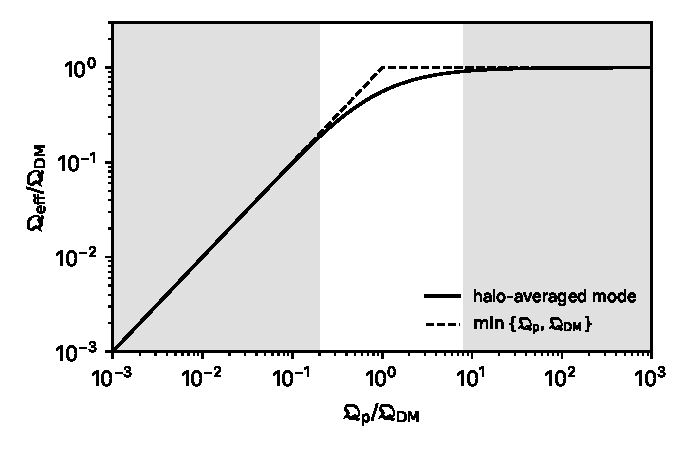
\includegraphics[width=0.8\linewidth]{figures/ch11/limit11_8b.pdf}
\captionof{figure}{Effective quality factor of a resonator mode in the halo field, \cref{eq:11.8-Qeff}, in units of $\mathfrak{Q}_{\mathrm{DM}} = 1.34\times10^6$, against the quality factor of the mode, $\mathfrak{Q}_{\mathrm{p}}/\mathfrak{Q}_{\mathrm{DM}}$, with the mode tuned to the frequency that maximizes it. Solid: \cref{eq:11.8-Qeff} with $F_\phi$ from the speed distribution of the standard halo of \cref{sec:1.2}; dashed: $\min\{\mathfrak{Q}_{\mathrm{p}}, \mathfrak{Q}_{\mathrm{DM}}\}$. Gray: $\mathfrak{Q}_{\mathrm{p}}/\mathfrak{Q}_{\mathrm{DM}} < 0.2$ and $> 7.9$, where the two agree within \SI{10}{\percent}. At $\mathfrak{Q}_{\mathrm{p}} = \mathfrak{Q}_{\mathrm{DM}}$ the prescription is 1.8 times too high.}\label{fig:11-limit-8b}
\par}
\smallskip
Where the widths of the mode and of the field are comparable, the signal is their convolution and neither width alone sets it; for records shorter than the coherence time the mean power is not a rate at all.
\end{limitbox}

The inputs that \cref{eq:11.8-Pn} needs are material and geometric. The elastic and piezoelectric tensors come from density-functional perturbation theory, and the shapes and frequencies of the modes of the actual body from finite elements. Add the shape factor $f_{\mathrm{sh}}$ of \cref{eq:11.8-shape} and the measured quality factor of the mode, which for acoustic resonators of this kind lies between $10^6$ and $10^{10}$~\cite{trickle2025piezoelectric}. A mode with $\mathfrak{Q}_{\mathrm{p}}$ above $10^7$ is in the narrow regime, where the signal is set by the field, not by the resonator. Its ring-down time, $\mathfrak{Q}_{\mathrm{p}}/\omega_n$, then exceeds the coherence time of the field, and the mean power of \cref{eq:11.8-Qeff} is reached only after many coherence times. How the signal builds up over shorter records, and how it fluctuates, is the coherent regime of \cref{sec:14.6}.

\subsection{Resonant-mass detectors}\label{sec:11.8-mass}

At masses of a peV to a neV the scalar of \cref{sec:11.8-gaas} does something else. Its coupling $g_{\phi ee}\phi\bar\psi\psi$ adds $-g_{\phi ee}\phi$ to the electron mass, and with $\phi = \phi_0\cos(m_\phi t)$, $\phi_0 = (2\rho_\chi)^{1/2}/m_\phi$, the electron mass oscillates, $\delta m_e/m_e = -g_{\phi ee}\phi/m_e$. A scalar coupled to $F_{\mu\nu}F^{\mu\nu}$ makes the fine-structure constant oscillate in the same way. Arvanitaki, Dimopoulos and Van Tilburg write both with dimensionless couplings normalized to the strength of gravity~\cite[Eqs.~(1), (3), (4)]{arvanitaki2016sound}. Such a field changes the size of every atom. The Coulomb Hamiltonian of electrons and clamped nuclei, \cref{eq:2.3-HC} with $M_\kappa \to \infty$, contains $\alpha$ and $m_e$ only through the Bohr radius $a_0 = 1/(\alpha m_e)$, which sets every length, and $\alpha^2m_e$, which sets every energy. The lattice constant is a fixed number of Bohr radii, and
\begin{equation}
  h_{\mathrm{mod}} \equiv \frac{\delta a}{a} = -\frac{\delta\alpha}{\alpha} - \frac{\delta m_e}{m_e} .
  \label{eq:11.8-h}
\end{equation}
The scaling fails only through physics that the Coulomb Hamiltonian leaves out. Relativistic corrections are of relative order $(Z\alpha)^2$ for the inner electrons. They add to $\dd\ln a/\dd\ln\alpha$ a term that fully relativistic calculations put at $-1.97\times10^{-2}$ for copper and $-2.2\times10^{-4}$ for silicon; the finite nuclear mass adds a dependence on the proton-to-electron mass ratio, $-1.12\times10^{-3}$ per unit fractional change for copper and $-0.86\times10^{-3}$ for silicon~\cite[Table~II]{pasteka2019material}. For a light crystal \cref{eq:11.8-h} holds to about $10^{-3}$.

A resonant-mass detector reads out such a change. It is a massive elastic body, a cylindrical bar or a sphere, of low internal loss, whose lowest mode is watched by a transducer at its own frequency. The detectors were built for gravitational waves, and the cryogenic ton-scale aluminum bars of the last generation ring near \SI{900}{Hz}~\cite{arvanitaki2016sound}, an energy of \SI{3.7}{peV}.

Why should an oscillating size excite a mode at all? A static change of $a$ excites nothing. The body simply takes its new equilibrium shape, with every material point $\vect{\xi}$ moved to $(1 + h_{\mathrm{mod}})\vect{\xi}$, and there is no wave. Write the displacement in the laboratory as $\vect{u}_{\mathrm{lab}} = \vect{u} + h_{\mathrm{mod}}(t)\,\vect{\xi}$, with $\vect{u}$ the displacement from the instantaneous equilibrium. The elastic stress responds to the strain relative to that equilibrium, $\sigma = C : (\nabla\vect{u}_{\mathrm{lab}} - h_{\mathrm{mod}}\mathbb{1}) = C : \nabla\vect{u}$, for a uniform $h_{\mathrm{mod}}$ in a cubic or isotropic body, with $C$ the elastic tensor. Newton's law holds in the laboratory, $\rho_T\ddot{\vect{u}}_{\mathrm{lab}} = \nabla\cdot\sigma$, and
\begin{equation}
  \rho_T\,\ddot{\vect{u}} = \nabla\cdot(C : \nabla\vect{u}) - \rho_T\,\ddot h_{\mathrm{mod}}\,\vect{\xi} .
  \label{eq:11.8-drive}
\end{equation}
The scalar acts as a body force $-\rho_T\ddot h_{\mathrm{mod}}\vect{\xi}$, the inertial force of the moving equilibrium. It is proportional to $\omega^2h_{\mathrm{mod}}$: the stiffness of the body never enters, and a slow modulation is followed adiabatically. Projected on a mode $\vect{u}_n$ of the body, the force is $F_n = -\ddot h_{\mathrm{mod}}\int\dd^3\xi\,\rho_T\,\vect{\xi}\cdot\vect{u}_n$. For a sphere of radius $R_{\mathrm{sph}}$ and mass $M_{\mathrm{sph}}$ only the radial modes $\vect{u}_n = \hat{\vect{r}}u_n(r)$ couple, and $F_n = -\ddot h_{\mathrm{mod}}M_{\mathrm{sph}}R_{\mathrm{sph}}J_n$ with $J_n = 3R_{\mathrm{sph}}^{-4}\int_0^{R_{\mathrm{sph}}}\dd r\,r^3u_n(r)$, which Arvanitaki and collaborators obtain by treating the modulus as a scalar gravitational wave with the curvature $\delta_{ij}\ddot h$~\cite[Eqs.~(7), (8)]{arvanitaki2016sound}.

A thin bar of length $L_{\mathrm{b}}$ and sound speed $c_{\mathrm{b}}$, free at both ends, shows the whole response in closed form. Along the bar, \cref{eq:11.8-drive} with $h_{\mathrm{mod}}\ee^{-\ii\omega t}$ has the solution $u_{\mathrm{lab}} = h_{\mathrm{mod}}\sin(k\xi)/[k\cos(kL_{\mathrm{b}}/2)]$, $k = \omega/c_{\mathrm{b}}$, which satisfies the free-end condition $\partial_\xi u_{\mathrm{lab}} = h_{\mathrm{mod}}$ at $\xi = \pm L_{\mathrm{b}}/2$. Measured from the instantaneous equilibrium, the end moves by
\begin{equation}
  u(L_{\mathrm{b}}/2) = \frac{h_{\mathrm{mod}}L_{\mathrm{b}}}{2}\Bigl(\frac{\tan x}{x} - 1\Bigr) , \qquad x = \frac{\omega L_{\mathrm{b}}}{2c_{\mathrm{b}}} = \frac{\pi}{2}\,\frac{\omega}{\omega_1} ,
  \label{eq:11.8-bar}
\end{equation}
with $\omega_1 = \pi c_{\mathrm{b}}/L_{\mathrm{b}}$ the lowest mode that couples. Below it, $\tan x/x - 1 \simeq x^2/3$, and the response is $(\pi^2/24)\,h_{\mathrm{mod}}L_{\mathrm{b}}(\omega/\omega_1)^2$, the $\omega^2$ of the drive. At each odd mode it resonates. Far above, the end stays where it was in the laboratory while the equilibrium moves, and the relative displacement tends to $-h_{\mathrm{mod}}L_{\mathrm{b}}/2$. The lowest mode alone, $u_1 = \sin(\pi\xi/L_{\mathrm{b}})$ with mass $M_{\mathrm{b}}/2$ and force $2\omega^2h_{\mathrm{mod}}M_{\mathrm{b}}L_{\mathrm{b}}/\pi^2$, gives $(4/\pi^2)h_{\mathrm{mod}}L_{\mathrm{b}}(\omega/\omega_1)^2/(1 - \omega^2/\omega_1^2)$; its low-frequency coefficient, $4/\pi^2 = 0.405$, falls short of $\pi^2/24 = 0.411$ by the higher odd modes, whose shares $4/\pi^2n^4$ sum to the difference.

\begin{limitbox}[Resonant-mass drive of a scalar][lim:11.8c]
A scalar that changes $\alpha$ or $m_e$ strains a body by $h_{\mathrm{mod}} = -\delta\alpha/\alpha - \delta m_e/m_e$ and drives its modes with the force $F_n = -\ddot h_{\mathrm{mod}}M_{\mathrm{sph}}R_{\mathrm{sph}}J_n$, proportional to $\omega^2$~\cite[Eqs.~(6)--(8)]{arvanitaki2016sound}.
\par\smallskip
{\centering
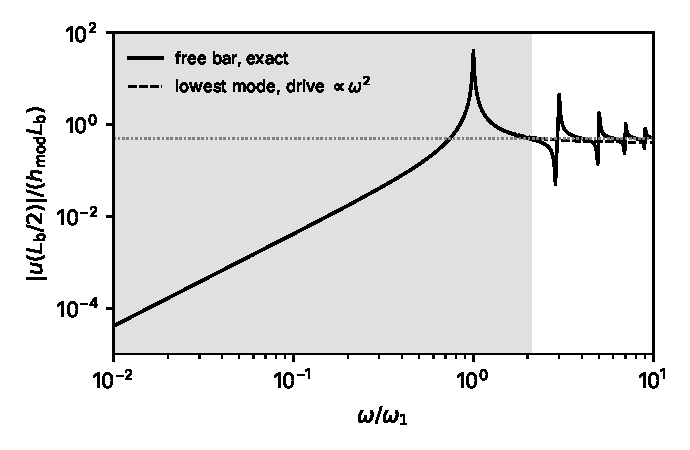
\includegraphics[width=0.8\linewidth]{figures/ch11/limit11_8c.pdf}
\captionof{figure}{Displacement of the end of a free bar from its instantaneous equilibrium, in units of $h_{\mathrm{mod}}L_{\mathrm{b}}$, against $\omega/\omega_1$. Solid: the exact response \cref{eq:11.8-bar}; dashed: the lowest mode alone with the $\omega^2$ drive. Every mode has the width $\omega_n/\mathfrak{Q}$ with $\mathfrak{Q} = 100$ for visibility (resonant-mass detectors reach $10^6$ to $10^7$). Dotted: the high-frequency limit $1/2$. Gray: $\omega < 2.1\,\omega_1$, where the lowest mode is within \SI{10}{\percent} of the exact response. The field is uniform over the bar while $m_\phi vL_{\mathrm{b}} \ll 1$. With $v = 10^{-3}$ and $c_{\mathrm{b}} = \SI{5}{km/s}$ this holds up to $\omega \approx 2\times10^7\omega_1$, far off scale.}\label{fig:11-limit-8c}
\par}
\smallskip
Above the lowest mode the higher modes and their antiresonances take over, and the response approaches the rigid limit, in which the body no longer follows its equilibrium.
\end{limitbox}
